\documentclass{article}
\usepackage[utf8]{inputenc}
\usepackage[T1]{fontenc}
\usepackage{lmodern}
\usepackage{graphicx}
\usepackage{listings}
\usepackage{amsmath}
\usepackage{multirow}
\usepackage{url}
\usepackage{textcomp}
\usepackage[normalem]{ulem}
\usepackage{colortbl}
\usepackage[usenames,dvipsnames,svgnames,table]{xcolor}
\usepackage{pgfplots}
\usepackage{pdfpages}
\usepackage{hyperref}

\definecolor{mygreen}{rgb}{0,0.6,0}
\definecolor{mygray}{rgb}{0.5,0.5,0.5}
\definecolor{myorange}{rgb}{0.58,0,0.82}


\title{Projet CSD 2018 }
\author{Flory Colin, Maussion Juliette, Renault Jean-Baptiste}
\date{Juin 2018}

\lstset{frame=tblr,breaklines=true,commentstyle=\color{mygreen},stringstyle=\color{orange},keywordstyle=\color{blue},numbers=left,extendedchars=true,inputencoding=utf8,showstringspaces=false}
\pgfplotsset{compat=1.15}




\begin{document}

\begin{titlepage}

    \begin{figure}
        \centering
        
\includegraphics[scale=0.3]{titre.png}
        \label{fig:titre}
    \end{figure}
    \maketitle
    \thispagestyle{empty}
    \begin{figure}
   \begin{minipage}[c]{.46\linewidth}
      
\includegraphics[scale=0.05]{logo_TNCY.png}
   \end{minipage} \hfill
   \begin{minipage}[c]{.46\linewidth}
      
\includegraphics[scale=0.13]{LogoUnivLorraine.png}
   \end{minipage}
\end{figure}
    
\end{titlepage}


\newpage

\null\thispagestyle{empty}\newpage
\setcounter{page}{1}
\renewcommand{\contentsname}{Sommaire}
\tableofcontents
\newpage


\section*{Introduction}     \par L'équipe ayant travaillé sur le projet présenté dans ce rapport est constituée de deux anciens élèves CPGE, Jean-Baptiste RENAULT et Juliette MAUSSION ainsi qu'un ancien élève de DUT informatique, Colin FLORY. Ce projet s'inscrit dans le module Langage C et Structure de Données.
\par Ce rapport a pour objectif de présenter notre démarche visant à obtenir une application de recommandation de films. Il débutera par un état de l'art des différents principes et techniques que nous avons mis en oeuvre pour mener à bien ce projet, un rappel sur le langage C, puis abordera la démarche suivie pour concevoir les différentes fonctionnalités de notre programme, pour conclure sur la gestion de projet.
\newpage


\section{Etat de l'art}
\subsection{Introduction}

\subsubsection{Pourquoi ?}

Les algorithmes de recommandation sont utilisés afin de soumettre à un utilisateur des items qu'il est susceptible d'apprécier lors de la recherche, ils servent ainsi à donner des suggestions à cet utilisateur en filtrant les résultats inappropriés afin que ce dernier puisse diminuer son temps de recherche. On peut retrouver ce type d'algorithmes lors d'une recherche dans un navigateur web, sur des sites d'achat en ligne ou encore sur des sites de streaming tels que Netflix\cite{eda}.

\subsubsection{Les informations nécessaires aux systèmes de recommandation}

Les systèmes de recommandation se basent sur les connaissances suivantes des utilisateurs et des items : la connaissance du profil des utilisateurs (leurs goûts, d'autres informations personnelles), le positionnement d'un utilisateur par rapport à d'autres, comme les similarités de comportement entre les utilisateurs; la connaissance de descripteurs des items à recommander, afin de pouvoir mettre en évidence les similarités entre les items.

Les appréciations des items par les utilisateurs peuvent être regroupés dans une matrice dite matrice d'usage, qui permet de faire correspondre à chaque couple (utilisateur \verb'u', item \verb'i') un score, qui dans notre cas correspond à une note.
 \begin{figure}[!h]
\begin{center}
\begin{tabular}{|c|c|c|c|c|}
\hline
&item 1&item 2&item 3&item 4\\
\hline
utilisateur 1&3&&5&1\\
\hline
utilisateur 2&2&4&&\\
\hline
utilisateur 3&&5&&\\
\hline
utilisateur 4&1&&3&5\\
\hline
\end{tabular}
\newline\newline
\caption{Matrice d'usage}
\end{center}
 \end{figure}

Les systèmes de recommandations peuvent être classés en trois grandes catégories : 
\begin{itemize}
    \item ceux utilisant un filtrage à base de contenu ;
    \item ceux utilisant un filtrage collaboratif ;
    \item ceux dits hybrides, utilisant les deux approches précédentes.
\end{itemize}


\subsection{Filtrage par le contenu}

\subsubsection{Principe}

Le filtrage par contenu repose sur le classement des items les plus similaires aux goûts d'un utilisateur, sans faire intervenir les autres utilisateurs, mais sur les particularités de chacun des items. Dans le cadre de notre projet, les attributs se traduisent par les différents genres des films, qui sont les acteurs, le directeur de production, la durée du film (des films de très longue durée peuvent être suggérés après le visionnage de l'un d'entre eux par exemple), voire même des tags, des thématiques plus éloignées des genres, grâce à l'accès aux résumés. 

Ce type de filtrage nécessite donc un minimum de connaissances des profils des utilisateurs, pour établir les goûts, la connaissance des items et la classification de ces items. En effet, la détermination d'un profil d'item permet des rapprochements item-item qui eux-mêmes permettent de se passer en partie des actions des autres utilisateurs. 

Ce filtrage se base sur les recherches que l'utilisateur aurait faites et sur les contenus qu'il aurait déjà parcourus. Il s'agit ensuite de classer ces requêtes selon leur proximité en utilisant par exemple les mots contenus dans la recherche ou dans les documents recherchés, mais aussi les mots qui ne sont pas contenus dans ces recherches (ce qui permet de savoir les résultats que l'utilisateur ne souhaite pas voir à priori).

\subsubsection{Les profils}

Le profil des items est un vecteur de score sur des attributs/descripteurs de l'item.

Le profil des utilisateurs est établi implicitement, par ses interactions avec les items, et explicitement par des questions directes. Ainsi, son profil implicite est déterminé grâce à la fréquence d'apparition d'items dans ses recherches, ou des mots-clés. Il est indiqué aussi que la fréquence de non-apparition est à prendre en compte: la non-apparition d'un mot dans une recherche peut être due à un choix de l'utilisateur. Ainsi le profil des utilisateurs est aussi un vecteur qui correspond aux mêmes attributs/descripteurs que les items; dont le score correspond à ses préférences.
\subsubsection{Approches}
L'approche la plus classique qui permet d'obtenir de bons résultats pour sa simplicité est l'approche vectorielle.
Elle est déterminée à partir d'une matrice de scores dont chaque ligne correspond à un descripteur et chaque colonne à un item (dans notre cas, on aurait les films/séries en colonnes et les attributs du type acteurs/genre/... en ligne).

\begin{figure}[!h]
\begin{center}
\begin{tabular}{|c|c|c|c|c|c|c|c|}
\hline
&Horror&Action&Drama&Comedy&Family&Romance&Fantasy\\
\hline
Film 1&&1&&1&&&\\
\hline
Film 2&1&1&&&&&1\\
\hline
Film 3&&1&&1&1&&\\
\hline
Film 4&&&1&&1&1&\\
\hline
\end{tabular}
\newline\newline
\caption{ Matrice I de classification}
\end{center}
\end{figure}

La matrice de classification permet donc de déterminer les spécificités d'un film. Ainsi, pour chaque film/série \verb'i' est associé le vecteur correspondant à la ligne \verb'i' de la matrice \verb'I', contenant toutes les informations connues sur le film, qui peuvent êtres communes à d'autres (on ne prend pas en compte ici du titre du film, du résumé).

De même, on peut déterminer un vecteur \verb'u' correspondant à l'utilisateur, qui somme tous les scores des items qu'il a déjà vu/dont il y a un score, suivant ses descripteurs.

Ce vecteur et la matrice de classification permettent de déterminer le vecteur profil \verb'p'. Ce vecteur permet de comparer pour chaque utilisateur les items qui se rapprochent le plus de ce qu'il a déjà apprécié. Il se calcule de la manière suivante : \verb'p = u.I' .

Le vecteur profil \verb'p' permet de calculer les distances de Pearson, qui séparent les items de celui-ci; les distances les plus petites étant celles dont les items se rapprochent le plus du profil de l'utilisateur. C'est à partir des calculs de distance que l'on peut faire un classement des items et ainsi fournir à l'utilisateur une recommandation. 

Pour calculer le coefficient de similarité de Pearson, on calcule le cosinus de l'angle entre les deux vecteurs : 

\[sim(p,i)=cos \alpha = \frac{p.i}{||p||\cdot||i||}\]

D'autres approches sont possibles, suivant des modèles d'apprentissage pour chaque utilisateur (réseau de neurones, arbre de décision, forêt aléatoire, SVM, etc).

La mise en place d'une validation de la recommandation par l'utilisateur permet d'accorder une plus grande confiance dans les scores de chaque items pour chaque utilisateur, permettant ainsi l'obtention de recommandations encore plus pertinentes par cette mise à jour dynamique.


\subsubsection{Avantages/Inconvénients}

Avantages :
\begin{itemize}
    \item L'algorithme est dynamique : plus l'utilisateur utilise le système, plus ce dernier est pertinent;
    \item Un nouvel arrivant via son profil qui est complété de manière explicite peut avoir des recommandations dès le début, moins pertinent que les recommandations qui observent son profil implicite.
    \item Permet la recommandation de nouveaux items.
\end{itemize}
Inconvénients : 
\begin{itemize}
    \item Redondance des thèmes proposés : les items non similaires à ceux déjà appréciés par l'utilisateur ne seront pas proposés;
    \item Problème du "nouvel arrivant" : Sans profil explicite, l'utilisateur ne se verra pas recommander de résultats pertinents s'il n'a pas encore utilisé le système;
    \item Nécessite beaucoup d'informations via les descripteurs sur les items et/ou les utilisateurs.
\end{itemize}

Ces inconvénients peuvent être limités grâce à la mise en place de recommandations pseudo-aléatoires en plus de celles déjà filtrées (inconvénient 1), grâce à des algorithmes de classification. On peut également désactiver le système de recommandation tant que l'on considère ne pas avoir suffisamment d'informations (inconvénient 2).

\subsection{Filtrage collaboratif}

\subsubsection{Principe}

Le filtrage collaboratif se base sur les similarités entre un profil d'utilisateur donné et les profils des autres utilisateurs.
Contrairement au filtrage par contenu, le contenu des items n'est pas considéré; le système de recommandation a besoin en revanche des préférences des autres utilisateurs pour pouvoir comparer les différents profils\cite{theseBC}. 

\subsubsection{Les profils}

Contrairement au filtrage par contenu, il faut connaître non seulement le profil de l'utilisateur, mais aussi celui de tous les autres. Il faut tout d'abord initialiser le profil (soit proposer des recommandations aléatoires puis rapprocher l'utilisateur avec un profil type, soit le rapprocher directement à d'autres utilisateurs grâce à ses informations personnelles : âge, nom, adresse,...).


\subsubsection{Approches}

Une approche assez classique est celle d'établir le voisinage de l'utilisateur. On commence tout d'abord par normaliser ligne par ligne la matrice d'usage\cite{diapo} en soustrayant à chaque score la valeur moyenne de chaque utilisateur (une ligne correspond à un seul utilisateur pour tous les items). Cette normalisation permet d'amoindrir les différences de notation entre les utilisateurs : il arrive fréquemment que certains notent au-dessus de la moyenne de notation constamment, d'autres à l'inverse sous-notent les items. 

Par exemple, pour la matrice d'usage donnée dans l'introduction, on obtient donc : 


\begin{figure}[!h]
\begin{center}
\begin{tabular}{|c|c|c|c|c|}
\hline
&item 1&item 2&item 3&item 4\\
\hline
utilisateur 1&0&&2&-2\\
\hline
utilisateur 2&-1&1&&\\
\hline
utilisateur 3&&0&&\\
\hline
utilisateur 4&1&&3&5\\
\hline
\end{tabular}
\newline\newline
\caption{Matrice d'usage normalisée}
\end{center}
\end{figure}

Comme pour le filtrage par contenu, on considère le vecteur profil de l'utilisateur \verb'A', cette fois-ci simplement extrait de la matrice normalisée, qui prend donc comme valeur les scores centrés des items. Il faut ensuite calculer pour chaque utilisateur la corrélation de Pearson, c'est-à-dire calculer le cosinus de l'angle séparant les vecteurs profils entre l'utilisateur \verb'A' considéré et chaque autre utilisateur. Ce calcul est le même que pour le filtrage par contenu en modifiant les vecteurs: 

\[sim(A,u)=cos~\beta = \frac{A.u}{||A||\cdot||u||}\]

Le score supposé pour un item \verb'i' et l'utilisateur \verb'A' est la moyenne pondérée des scores suivant les utilisateurs qui ont vu l'item et l'item en question. Le score pris pour chaque couple \verb'{utilisateur, item}' provient évidemment de la matrice normalisée et non de la matrice d'usage non modifiée.
\[score(utilisateur~A, item~i) = \sum_{u} \frac{sim(A,u)\cdot score(u,i)}{\sum_{u} |sim(A,u)|}\]

On trouve dans la littérature que l'on peut amplifier les similitudes en portant à la puissance 2.5 la corrélation de Pearson : \[score(utilisateur~A, item~i) = \sum_{u} \frac{sim(A,u)^{2.5}\cdot score(u,i)}{\sum_{u} ~|sim(A,u)^{2,5}|}\]

Il reste ensuite à faire ce calcul avec tous les items. La complexité de cet algorithme est de $O(mnx)$ avec \verb'm' le nombre d'utilisateurs, \verb'n' le nombre d'item, et \verb'x' le nombre d'articles notés par utilisateur. On remarque que cet algorithme a donc une couverture limitée; son utilisation peut être appliquée sur un nombre déterminé d'utilisateurs à comparer lorsqu'il y a un trop grand nombre d'utilisateurs.
L'avantage de cette méthode est aussi d'éviter les profils qui ont pour objectif d'orienter les choix des autres utilisateurs.
\newline

Il est possible de filtrer par regroupement (clustering). C'est par exemple le cas pour des films du même opus. Le principe est de regrouper les items de la même catégorie. Pour déterminer un score supposé, lorsque l'utilisateur a vu au moins un des items du cluster, le score est égal à la moyenne. S'il n'y a aucune information sur le cluster considéré, le score est calculé de la même manière que ci-dessus, en partant non de la matrice d'usage de l'introduction, mais d'une matrice utilisateurs-clusters qui lui est très semblable.
L'avantage du clustering est de réduire les calculs et de proposer des suggestions cohérentes au visionnage d'opus. 


 \begin{figure}[!h]
\begin{center}
\begin{tabular}{|c|c|c|c|c|}
\hline
&item 1 et 2&item 3&item 4, 5 et 6&item 7\\
\hline
utilisateur 1&3&&5&1\\
\hline
utilisateur 2&2&4&&\\
\hline
utilisateur 3&&5&&\\
\hline
utilisateur 4&1&&3&5\\
\hline
\end{tabular}
\newline\newline
\caption{Matrice utilisateurs-clusters}
\end{center}
\end{figure}

Une autre approche fréquemment rencontrée dans la littérature est celle des stéréotypes, c'est-à-dire considérer que la création d'un profil initial d'utilisateur est un problème de classification.



Lorsque l'utilisateur n'a pas assez noté d'item, ce qui est le cas lorsqu'on se retrouve avec un nombre d'item vu entre 0 et 3, on peut retourner à la stratégie de recommandation non personnalisée en faisant appel à des classements comme les "Top 10".\cite{theseClu} 

\subsubsection{Avantages/Inconvénients}

Avantages : 
\begin{itemize}
    \item On se dispense des descripteurs sur les items/utilisateurs;
    \item La dimension psychologique de l'utilisateur est mise en place par ce type de filtrage, ce qui rend les résultats plus pertinents.
\end{itemize}
Inconvénient :
\begin{itemize}
    \item Manque la notion de thème;
    \item Subit un démarrage à froid, manquant de données à ses débuts;
    \item Temps de calcul considérable;
\end{itemize}
Cet inconvénient peut être évité en utilisant également une classification thématique dans la recommandation : c'est la méthode hybride.

\subsection{Méthodes hybrides}

\subsubsection{Principe}

Il existe deux types de méthodes hybrides :
\begin{itemize}
    \item Combiner les ensembles de recommandations fournies par le filtrage par contenu et le filtrage;
    \item Regrouper les notions basées sur le filtrage par contenu et le filtrage collaboratif afin de construire un nouveau modèle.
\end{itemize}
On peut combiner les ensembles de recommandations par pondération, commutation, cascades, etc.
Aussi, une simple combinaison linéaire des scores retournés par les différentes approches améliore significativement les résultats.

Il existe aussi d'autres méthodes, non seulement hybrides, mais qui prennent en compte des informations diverses telles que la dimension psychologique, les données sociales démographiques, les logs de navigation Web, l'âge, le métier, le genre, les commentaires, les avis, pour chaque utilisateur, mais aussi la météo, l'heure, en considérant que tous ces paramètres peuvent influencer à un moment donné le choix d'un utilisateur vers un item plutôt qu'un autre.

\subsubsection{Avantages/Inconvénients}

    Avantage : cette technique permet de pallier les limites des recommandations par contenu et collaboratif en les combinant.
    \newline
    \\ Inconvénient : Il n'est pas facile de pondérer ou d'évaluer la pertinence entre les deux premières méthodes.

\subsection{Évaluation d'un système de recommandation}

    Les systèmes de recommandation sont évalués selon deux principaux critères :
\begin{itemize}
\item La précision de la prédiction de préférence
\item La couverture des prédictions (quantité)
\end{itemize}
    L'objectif d'un système de recommandation est de trouver un compromis entre ces deux critères pour avoir des résultats pertinents.

    On peut évaluer la précision par le calcul de l'erreur moyenne absolue\cite{diapo2}, c'est-à-dire la moyenne des différences des notes prédites avec les notes réelles : 
    \[e = \frac{\sum_{i=1}^{N}|p_i-a_i|}{N}\]


\newpage




\section{Rappels sur le langage C}
    Le langage C était un nouveau langage pour la plupart des membres du groupe. Ce langage nous a posé deux problèmes : les pointeurs et la gestion de la mémoire. Ces deux points seront expliqués dans les paragraphes suivants pour une meilleure compréhension du compte-rendu.\\
\subsection{Les pointeurs}
    Les pointeurs sont des éléments clefs du langage C. Le principe d'un pointeur est, comme son nom l'indique, de pointer vers un élément. Cet élément est une adresse mémoire ce qui nous permet d'accéder directement à la couche basse de l'ordinateur.
    \par Les pointeurs sont typés, cela veut dire qu'ils pointent sur une adresse mémoire de la taille du type. De plus, le langage C introduit l'arithmétique des pointeurs qui permet, quand on incrémente un pointeur, de ne pas l'incrémenter d'un octet mais de la taille du type pointé. Cela nous permet d'utiliser les pointeurs comme des tableaux typés. Cela veut dire que si l'on incrémente de 1 un pointeur de caractères alors on passera au caractère suivant dans le tableau.
    \par L'utilisation des pointeurs nous impose d'être minutieux dans notre façon de programmer, car si l'on sort de la taille attribuée au pointeur alors on s'aventure dans des zones mémoires non reservé et qui, au mieux, nous donnerons des résultats incohérents et au pire, des erreurs de segmentation (segmentation fault).
    
    \begin{figure}[!h]
    \centering
    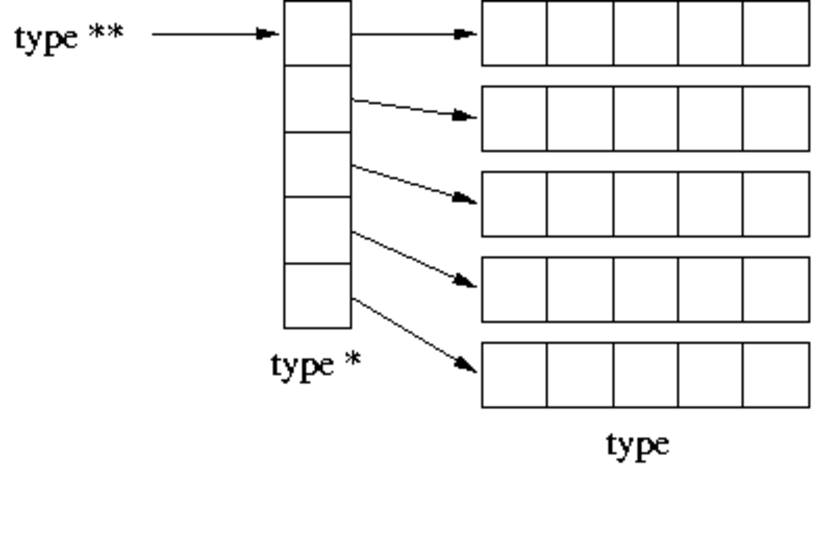
\includegraphics[scale=0.7]{Tableau.pdf}
    \caption{Représentation d'un pointeur de pointeur de caractère}
    \label{fig:my_label}
    \end{figure}

    \par Néanmoins il ne faut pas confondre l'astérisque situé après le type d'une variable et l'astérisque avant cette dernière. Si l'astérisque est avant, on parle alors de l'adresse de la variable.
    
\subsection{La gestion de la mémoire}
    En C une partie de la mémoire peut-être réservée à l'aide la fonction malloc(int Arg1). Cette fonction renvoie un pointeur vers une zone mémoire de taille Arg1. Il est important de toujours réserver la mémoire quand on utilise un pointeur pour éviter que l'ordinateur ne modifie des informations dans ces zones qui nous sont utiles. 
    \par Les zones réservées ne sont pas vides ! Elles sont remplies des informations qui s'y trouvaient précédemment. Une fois utilisées, les zones mémoires utilisées doivent être libérées à l'aide de la fonction free() qui prend en paramètre le pointeur à libérer.  

\newpage


\section{Parseur de document}
\subsection{Pourquoi ?}

    Nous avons décidé de créer un parseur de document ( fichier parseur.c ) pour pouvoir utiliser les différentes informations qui nous sont fournies dans le document texte BDCSD.txt. Ceci nous permet d'avoir une base de film de taille respectable pour pouvoir ainsi directement travailler sur la recommandation de film et l'affichage graphique.\\
    \par L'objectif principal lors de la création du parseur était de le faire le plus souple possible pour que les limites imposées à un document soit minimes tout en obtenant l'entièreté des informations.\\
    Un intérêt particulier a été porté sur l'utilisation optimale de la mémoire pour qu'à chaque variable soit alloué la taille correspondant parfaitement à ses besoins.\\

\subsection{Fonctionnement}
    Une fois le fichier passé en paramètre ouvert, notre algorithme itère sur chacune des lignes jusqu'à  trouver un nombre au début. Ce chiffre correspond à l'id du film et nous indique le début d'un nouveau film :\\
    On récupère le titre, l'année et le type du film sur la même ligne:
    \begin{itemize}
        \item Le titre se trouve entre le point qui suit l'id et la parenthèse ouvrante de l'année.
        \item L'année correspond aux 4 chiffres récupérés après la parenthèse ouvrante
        \item Le type d'une oeuvre est un film par défaut, sauf si la parenthèse de l'année ne ferme pas 5 caractères après son ouverture.Le type est symbolisé par un chiffre qui vaut 1 si c'est une série TV et 0 si c'est un film.
    \end{itemize}
    \par On parcourt les lignes suivantes à la recherche d'une lettre, qui indique la position du synopsis du film.
    \\
    \par Une fois le synopsis obtenu, on passe à la ligne suivante et l'on teste si ce film a un directeur de référencé. Pour cela on teste les 8 premières lettres et si ces lettres correspondent exactement à "Director" on récupère le ou les directeurs qui suivent. Si jamais il n'y a pas de directeur on utilise une valeur par défaut qui est : "director non reference"\\ 
    \par Pour terminer, on parcourt les dernières lignes pour récupérer les acteurs et les genres.
    \par Dans ces dernières lignes les acteurs et les genres sont séparés soit par une virgule ( pour les acteurs ) ou par un pipe ( pour les genres ).
    \par Après avoir récupéré tous les genres, il se peut que la durée du film soit présente, cette dernière est toujours accompagnée d'un point à la fin. C'est à cela qu'on identifie la durée du film, si jamais aucune durée n'est trouvée on utilise la valeur par défaut -1;\\
    

\subsection{Règles de bon fonctionnement}
    Pour que les informations soient bien prises en note, le fichier texte doit donc suivre ce schéma type:\\ \\
    \underline{ID} Titre du film \underline(année TV Series)(l'année doit être écrite avec 4 chiffres)\\
    Description.\\
    \underline{Director :} Nom du ou des directeurs ( séparés par une virgule )\\
    \underline{With :} Nom du ou des acteurs ( séparés par une virgule )\\
    Genre1 | Genre2 | ... | GenreN X \underline{mins.} ( la durée est optionnelle )\\ \\
    \par tout les éléments \underline{soulignés} sont obligatoires pour que toutes les informations soit prises en compte par le parseur.\\
    Le document "BDCSD.txt" fournis à l'intérieur de notre projet a été adapté aux besoins du parseur pour que l'entièreté des informations soit prise en compte.
    
\subsection{Remarque}
    Cette partie du projet n'est pas particulièrement compliquée, mais a posé beaucoup de problèmes et a demandé beaucoup de temps. Cela est en partie dû au fait que c'était la première étape de programmation du projet et donc celle sur laquelle les erreurs basiques se sont faites. De plus l'architecture globale du parseur fut entièrement changée au cours du projet, car je (Colin FLORY) n'étais pas totalement satisfait de la gestion de la mémoire qui, initialement était sur des tableaux de caractères de taille fixe ( 1000 caractères ), mais de peur que cela pose problème pour la suite du projet, l'entièreté de la mémoire s'adapte dorénavant à la taille des éléments trouvés.  

\newpage









\section{Structures de données}
\subsection{film}
    \begin{lstlisting}[language=C]
typedef struct film{
 int type;
 int annee;
 char* titre;
 char* description;
 char** acteurs;
 char** genres;
 char** director;
 int duree;
 int nbAct;
 int nbGenre;
 int nbDirector;
 int id;
}film;
    \end{lstlisting}
\subsubsection{Intérêt de la structure}
    La création d'une structure film est un élément inévitable du projet. Cette dernière est très importante, car elle contient l'entièreté des informations relatives aux films. Elle facilite donc la sauvegarde des informations et les rends facilement accessibles pour le reste du projet.
\subsubsection{Fonctions}
    Dans ce paragraphe, seules les fonctions les plus utilisées et les plus pertinentes de la structure seront traitées
    \begin{itemize}
        \item \textit{ film* film\_create() }: renvoie un pointeur vers une structure film prête à l'utilisation ( éléments initialisés à une valeur par défaut et les pointeurs à NULL ).
        \item \textit{film* film\_ajout(film* f,char* titreA, char* descriptionA,int typeA,int dureeA,int id,int annee)}: ajoute les informations de taille fixe ( différent des genres,des acteurs et du/des réalisateurs ) dans le film f passé en paramètre.
    \item \textit{film* film\_ajout\_acteur(film* f, char* director)} : ajoute un acteur au film.\\
    Les acteurs des films sont stockés dans une variable, un pointeur de pointeur de caractères (tableau de tableau). Or un problème apparait lorsque l'on souhaite ajouter un nouvel acteur au film, la taille attribuée à la variable risque d'être trop petite.\\
    C'est pour éviter cela que cette fonction a été conçue. On crée donc un nouveau tableau de tableau de même taille que le précédent + la taille d'un pointeur (1). On obtient donc un tableau capable d'accueillir un directeur de plus. On copie toutes les informations du tableau initial vers le nouveau tableau (2). On ajoute le nouvel acteur (3). On libère l'espace mémoire de l'ancienne variable, on alloue la bonne taille à cette dernière et on copie les informations de la variable temporaire (4) . On libère la variable temporaire (5) .

    \begin{lstlisting}[language=C]
temporaire=malloc((f->nbAct+1)*sizeof(char*));  (1)
if(temporaire==NULL){
 printf("Echec allocation acteur\n");
 return f;
}
for(i=0;i<f->nbAct;i++){                        (2)
 temporaire[i]=strdup(f->acteurs[i]);
 if(temporaire[i]==NULL){
  printf("Echec allocation acteur\n");
 }
}
temporaire[f->nbAct] = strdup(acteur);          (3)
if(temporaire[f->nbAct]==NULL){
 printf("Echec allocation2 acteur\n");
 return f;
}
for(i=0;i<f->nbAct;i++){                        (4)
 free(f->acteurs[i]);
}
free(f->acteurs);
f->acteurs=malloc((sizeof(char*)*(f->nbAct+1)));
for(i=0;i<f->nbAct+1;i++){
 f->acteurs[i]=strdup(temporaire[i]);
 if(f->acteurs[i]==NULL){
  printf("Echec allocation acteur\n");
 }
}
for(i=0;i<f->nbAct+1;i++){                      (5)
 free(temporaire[i]);
}
    \end{lstlisting}
    Cette fonction est déclinée pour les directeurs et les genres.
    
        \item \textit{void film\_copie(film* destination,film* source)}: copie toutes les informations du premier film vers le second.\\
    Cette fonction est très utile, car elle permet d'obtenir une copie parfaite d'un film, permettant d'être utilisés par un autre pointeur sans risque de perte d'informations.
    
        \item \textit{void film\_free(film* f)}: libère l'entièreté de l'espace mémoire attribué à un film.
    \end{itemize}



    \subsection{tableFilm}
    \begin{lstlisting}[language=C]
typedef struct tableFilm{
 int clef;
 struct tableFilm* suivant;
 struct tableFilm* precedent;
 film* valeur;
}tableFilm;
    \end{lstlisting}
    \subsubsection{Intérêt de la structure}
    Cette structure est là pour regrouper l'ensemble des films.\\
    C'est une liste doublement chainée, les avantages de ce type de structure est de ne pas avoir à gérer d'espace mémoire comme dans la structure film lors de l'ajout d'un film. Mon choix s'est porté sur une liste doublement chainée pour pouvoir se déplacer facilement d'un film à l'autre. Malheureusement, par manque de temps, cela ne fut jamais utilisé.\\
 \begin{figure}[!h]
    \centering
    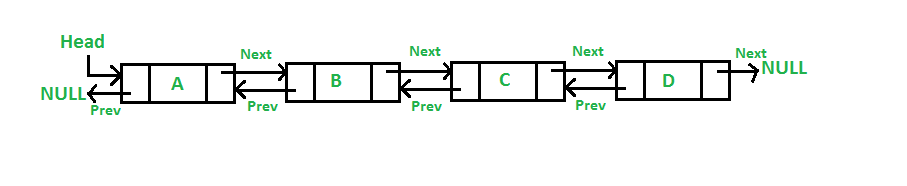
\includegraphics[scale=0.6]{DLL1.png}
    \caption{Représentation d'une liste doublement chainée}
    \label{fig:my_label}
\end{figure}
    \par On peut également observer la présence d'une variable clef à chaque noeud de la structure. Cette clef est un nombre correspondant au titre du film une fois passé dans notre fonction de hashage. Cette clef permet donc d'identifier très rapidement si un film a le même titre que celui du noeud. Le gain de temps est néanmoins minime. Ce point de la structure a donc été ajouté par simple curiosité de ma part ( FLORY Colin ). Son introduction durant le cours de Structure de Données et mon intérêt personnel pour la cryptographie ( malgré des connaissances vagues ) m'ont donc poussé à l'intégrer dans notre projet.
\subsubsection{Fonctions}
    \begin{itemize}
        \item \textit{tableFilm* createTableFilm()}: renvoie un pointeur vers une nouvelle structure.
        \item \textit{void tf\_ajoutFilm(tableFilm* tf, film* f)}: ajoute un film dans la tableFilm fournie.\\
    Les films sont ajoutés dans l'ordre croissant de leurs clefs. La fonction est très classique et reprends grandement ce qui a été vu en cours de SD.
        \item \textit{int tf\_getClef(film* f)}: retourne la clef correspondant au film.\\
    La fonction de hashage est une copie de celle utilisée par Java\cite{hashJava}. N'ayant pas de connaissances approfondies sur le sujet, l'utilisation de l'algorithme d'une si grosse structure est un choix sûr.
        \item \textit{film* tf\_getFilmByClef(tableFilm* tf,int clef)}: retourne le film correspondant à la clef.
        \item \textit{void libererMemoireTableFilm(tableFilm* tf)}: libère l'entièreté de la mémoire attribuée à la structure
    \end{itemize}
\medbreak
\subsection{matriceNote}
    \begin{lstlisting}[language=C]
typedef struct matriceNote{
 char* element;
 int valeur;
 struct matriceNote* suiv;
}matriceNote;
\end{lstlisting}

\subsubsection{Intérêt de la structure}
    Cette structure avait pour objectif d'être une matrice de distance entre les films. La distance correspondant à la similarité entre deux films, plus la distance est courte plus les films sont proches. Malheureusement, par manque de temps cela n'a pas pu être réalisé et une autre méthode a été choisie ( voir paragraphe 4.4 ). Cette matrice contient donc un élément, une valeur et un pointeur vers la structure suivante. Élément correspond à un aspect d'un film comme un genre ou un directeur. Valeur est la somme des notes attribuées aux films ayant cet élément. Le pointeur vers la structure permet de faire fonctionner le tout comme une liste simplement chainée. Les listes simplement chainées ont un fonctionnement similaire aux listes doublement chainées, mais sans le pointeur vers le noeud précédent.
    
\subsubsection{Fonctions}
    \begin{itemize}
        \item \textit{matriceNote* newMatrice()}: renvoie un pointeur vers une nouvelle matriceNote.
        \item \textit{void freeMatrice(matriceNote* mn)}: libère la mémoire.
        \item \textit{void ajoutMatrice(matriceNote* mn, char* nom, int valeur)}: ajoute en fin de liste un nouveau noeud avec les informations passées en paramètre.
    \end{itemize}
    

    
    
\subsection{Utilisateur}
    \begin{lstlisting}[language=C]
typedef struct utilisateur{
 char* nomUtilisateur;
 int clefPassword
 filmNote* premierFilm;
 filmReco* premierReco;
}utilisateur;
\end{lstlisting}

\subsubsection{Intérêt de la structure}
    Utilisateur est la structure comprenant toutes les informations utiles sur un utilisateur: nomUtilisateur et clefPassword sont deux éléments qui aurait permis d'avoir une série de profil et ainsi de se souvenir des préférences de chacun entre plusieurs utilisations. De plus la fonction de hashage créé précédemment aurait permis de chiffrer le mot de passe et ainsi de ne pas le rendre accessible directement dans les fichiers. \par Néanmoins par manque de temps, encore une fois, ces éléments intéressants ne sont pas intégrés au projet. Premierfilm et premierReco pointent respectivement vers le premier film noté par l'utilisateur et le premier film recommandé pour ce dernier.
\subsubsection{Fonctions}
    \begin{itemize}
        \item \textit{utilisateur* createUtilisateur(char* nom)}: renvoie un pointeur vers un nouvel utilisateur
        \item \textit{void utilisateur\_ajoutReco(filmReco* fr,film* f)}: ajoute un film recommandé pour l'utilisateur. Même principe pour \textit{void utilisateur\_ajoutFilm}, mais avec une note correspondant au film à ajouter.
    \end{itemize}
    filmNote et filmReco sont deux simples listes chainées.

\newpage





\section{Système de recommandation}
\subsection{Notation des films}
    La notation des films est un élément essentiel de notre système de recommandation par contenu. Les notes servent à savoir si un film a été apprécié par l'utilisateur et donc si des films semblables risquent de lui plaire également.
    \par Une série de 20 films choisis aléatoirement sont présentés à l'utilisateur et il doit leur attribuer une note comprise entre 0 et 10. Les films proviennent de la structure tableFilm qui contient l'ensemble des films et qui est remplie au cours du parsing du fichier texte de données.
\subsection{Algorithme de recommandation}
    Malgré les différentes formules et étapes inhérentes a une recommandation par contenu exposés dans l'état de l'art notre algorithme ne les suit qu'approximativement. La raison à cela est un manque de temps au cours du projet. 
    \par Notre algorithme essaye donc de se rapprocher de ce qui est écrit dans l'état de l'art, mais dans une version plus simple. L'objectif de l'algorithme est, en s'appuyant sur les films notés, attribuer un poids à chaque élément d'un film noté, le poids étant plus important si le film a été bien noté ou si cet élément revient souvent dans les films appréciés.
    
\subsection{Films recommandés}
    Une fois un poids attribué à chaque élément de tous les films notés, on compare tous les films de notre base avec notre matrice de note et on garde les 5 films obtenant le poids le plus fort.
    \par Ces films recommandés sont stockés pour chaque utilisateur dans l'espoir de pouvoir continuer le projet plus tard et ainsi garder en mémoire les films recommandés et demander à l'utilisateur s’ il a apprécié ces titres ainsi pouvoir changer rapidement son profil utilisateur.\\
    
\subsection{Remarques}
 Cette façon de faire présente de nombreux problèmes : 
    \begin{itemize}
        \item L'algorithme va privilégier les films avec beaucoup d'éléments, ces derniers vont emmagasiner beaucoup de poids et vont être prioritaire aux films avec moins d'éléments, mais correspondant plus aux attentes de l'utilisateur ( c'est pour cela que les mêmes films ressortent souvent).
        \item Les films proposés n'évolueront que très peu, si l'utilisateur décide de re noter certains films l'algorithme n'en tient pas compte.
        \item Le système de recommandation collaboratif n'est pas implémenté.
        \item L'algorithme ne peut reconnaitre la suite d'un film ( un numéro derrière le titre ou un mot clef tel que : "le retour" ) et ainsi le proposer si l'utilisateur a bien aimé l'original.
    \end{itemize}
    Cette partie du projet est un élément central et essentiel qui aurait mérité d'être plus approfondi. Néanmoins la présence d'un algorithme, certes imprécis et avec beaucoup de défauts, nous permet de tester tout le reste du projet et d'avoir un rendu final respectant tout les critères du cahier des charges.
    \par Si le projet se voit prolongé dans le temps, le système de recommandation devra être l'élément principal sur lequel travailler
\newpage



\section{Interface Graphique}
Nous avons codé l'interface graphique grâce à la librairie gtk+. Nous avons réalisé trois interfaces principales : l'interface de connexion, l'interface de sélection et l'interface de recommandation. Trois fenêtres sont gérées par la deuxième interface.
\noindent
\\ Nous avons décidé de nous concentrer sur la librairie gtk+ et de ne pas utiliser Glade afin de maîtriser correctement gtk+ (nous avons vu sur certains forums que Glade serait essentiellement conseillé à des utilisateurs qui connaissent déjà bien la librairie gtk+ et son fonctionnement).

%\renewcommand{\contentsname}{Sommaire}
%\tableofcontents

%\newpage
\subsection{Interface de Connexion}

\begin{figure}[h]
    \centering
    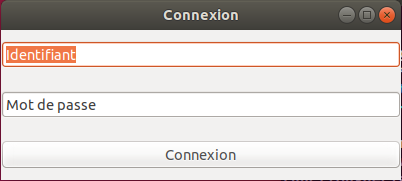
\includegraphics[scale=0.8]{InterfaceConnexion.png}
    \caption{Fenêtre de connexion}
    \label{SMART}
\end{figure}

\subsubsection{Le principe}

Nous avons voulu, à l'aide de cette interface, montrer une fenêtre qui demanderait à l'utilisateur son identifiant et son mot de passe, et qui passerait a la deuxième interface si les identifiants sont bons et si l'utilisateur appuie sur le bouton confirmer. Nous avons relié les identifiants à une structure utilisateur, mais ne leur avons pas associé de mot de passe (l'entrée dans la section mot de passe ne stocke donc pas ce que l'utilisateur rentre, et l'utilisateur n'est pas sauvegardé une fois l'algorithme terminé).

\subsubsection{En détail}

On définit les Widgets fenêtre,entrée d'identifiant, entrée de mot de passe, bouton de confirmation et une boite verticale.
\noindent
\\ On initialise gtk avec les paramètres argc et argv de la fonction main, on fait les réglages de la fenêtre (titre, taille ...).
\noindent 
\\ On ajoute ensuite la boite verticale (initialisée au préalable) dans la fenêtre et on insère dans cette boite verticale les deux entrées texte et le bouton (qu'on a assimilé au texte "Connexion").
\noindent 
\\ On crée enfin une connexion entre une fonction connexion-app (qui va effacer cette fenêtre et lancer la suivante, stocker l'identifiant mis en entrée dans une structure utilisateur) et le bouton "Connexion".
\noindent
\\ On montre la fenêtre.

\subsection{Interface de Sélection}

\begin{figure}[h]
    \centering
    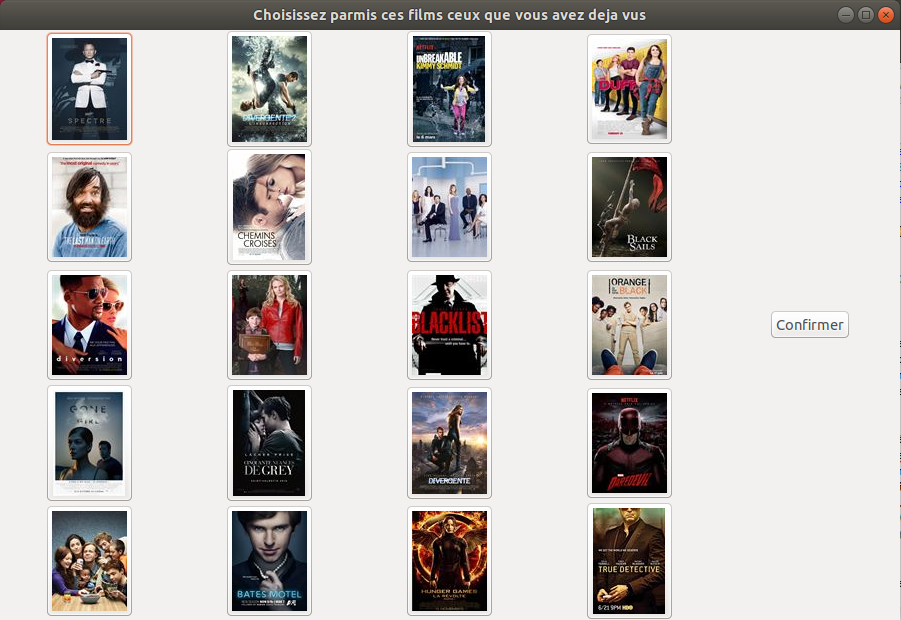
\includegraphics[scale=0.4]{InterfaceSelection.png}
    \caption{Fenêtre de sélection}
    \label{SMART}
\end{figure}

\subsubsection{Le principe}

\noindent
\\ Nous avons voulu créer une fenêtre qui permet à l'utilisateur de sélectionner parmi une sélection aléatoire de 20 films ceux qu'il a déjà vus et de les noter. Nous avons également considéré qu'il fallait que l'utilisateur sélectionne un nombre minimal de films, le cas échéant, une petite fenêtre d'erreur s'ouvre. Lorsqu'un film est sélectionné, une fenêtre de notation s'ouvre demandant d'entrer un entier entre 1 et 10, vérifiant que la note admet cette condition et la stocke. Une fois les films sélectionnés, l'appui sur un bouton "Confirmer" permet de passer à la fenêtre de recommandation.

\subsubsection{Les fonctions utilisées}
\noindent
\\ On définit le tableau film ainsi que 20 variables chemin[i] dans lesquelles on stocke le chemin vers le dossier PicturesFilms (où sont rangées les images en .jpg).
\noindent
\\ On crée une table de films et on la remplit avec les informations contenues dans BDCSD.txt (informations sur les films). On crée un entier n aléatoirement entre 0 et la taille de l'arbre -20.
\noindent
\\ On rentre dans le tableau films les noms des films d'indice n+i pour i allant de 0 à 19.
\noindent
\\ On concatène chaque chemin avec les éléments du tableau films. On concatène encore avec ".jpg" afin d'avoir dans les variables chemin[i] les chemins vers les images correspondant aux images des films sélectionnés précédemment.
\noindent
\\ On initialise la fenêtre et les boites (5 verticales et une horizontale). On insère la boite horizontale dans la fenêtre et les boites verticales dans la boite horizontale.
\noindent
\\ On définit 20 Widgets Image avec les 20 chemins construits précédemment, on insère ces images dans 20 boutons distincts. Ces boutons sont eux-mêmes insérés dans les 4 boites verticales les plus à gauche, on insère un bouton confirmer dans la boite verticale la plus à droite.
\noindent
\\ On crée ensuite 20 fonctions (chacune connectée à un bouton d'image) qui vont lancer une fenêtre de notation pour recueillir la note que l'utilisateur aura rentrée et va la stocker avec le film correspondant dans la structure utilisateur.
\noindent
\\ On crée une fonction verif() qui ouvre la fenêtre d'erreur si le nombre de films sélectionnés est inférieur à l'entier attendu, qui ferme la fenêtre et ouvre la fenêtre de recommandation sinon (en passant en arguments l'utilisateur et la table de films).
\noindent
\\ On montre la fenêtre.

\subsubsection{Les fenêtres intermédiaires qu'elle ouvre}
 Comme nous l'avons vu précédemment, certaines actions de l'utilisateur sur la fenêtre de sélection peuvent ouvrir deux autres fenêtres : une fenêtre d'erreur ou une fenêtre de notation :


\begin{itemize}
    \item La fenêtre de notation :
    \begin{figure}[h]
        \centering
        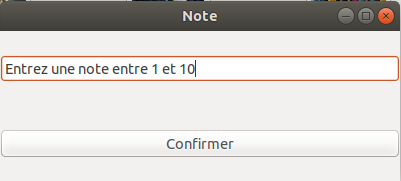
\includegraphics[scale=0.8]{InterfaceNote.png}
        \caption{Fenêtre de notation}
    \label{SMART}
    \end{figure}
    \\ On initialise la fenêtre et la boite verticale, on insère cette boite dans la fenêtre.
    
     On insère dans cette boite une entrée (préremplie avec le texte "Entrez une note entre 1 et 10") et un bouton "Confirmer".\\
    
    On connecte le clic sur le bouton à la fonction confirmationNote() qui renvoie la conversion en entier de la valeur en entrée et ferme la fenêtre si c'est bien un entier entre 1 et 10, qui exécute la fonction nonEntier() sinon.\\
    
    La fonction nonEntier() réécrit dans l'entrée un message indiquant à l'utilisateur que son entrée est invalide et spécifiant l'entrée attendue.\\
    
    \item La fenêtre d'erreur :
    \\ Cette fenêtre ne comporte qu'un bouton "fermer" et un label (indiquant que le nombre de films sélectionnés est insuffisant). On initialise la fenêtre, on insère la boite verticale dans la fenêtre puis le label et le bouton dans la boite. On connecte le bouton avec la fonction quitter() qui efface cette fenêtre.
    
    \begin{figure}[h]
        \centering
        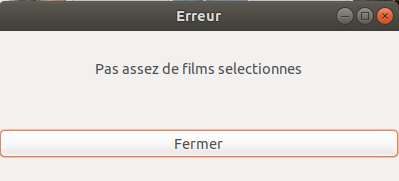
\includegraphics[scale=0.8]{InterfaceErreur.png}
        \caption{Fenêtre d'erreur}
    \label{SMART}
    \end{figure}
\end{itemize}




\subsection{Interface de Recommandation}

    \begin{figure}[h]
        \centering
        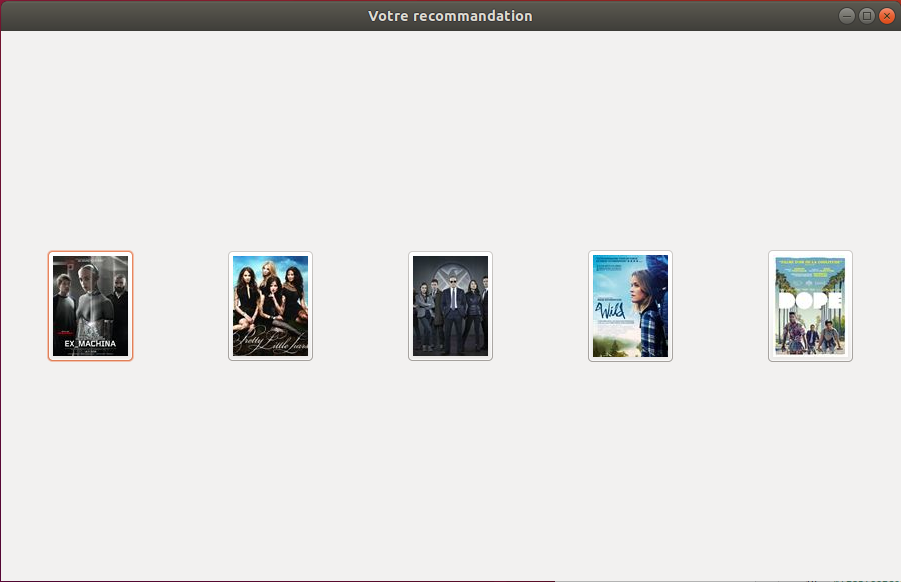
\includegraphics[scale=0.4]{InterfaceRecommandation.png}
        \caption{Fenêtre de recommandation}
    \label{SMART}
    \end{figure}

\subsubsection{Le Principe}

Enfin, nous avons voulu afficher une fenêtre contenant les recommandations assimilées à la sélection qui a eu lieu dans la fenêtre précédente. Il n'y a donc plus besoin de connexions pour aucun Widget de cette fenêtre (mis à part la croix en haut à gauche pour fermer la fenêtre).

\subsubsection{Les fonctions utilisées}

On définit la taille/le titre de la fenêtre. On définit les différents Widgets (5 images, 5 boutons qu'on associera aux images et 5 boites verticales).
\noindent
\\ On définit un tableau de caractères recommandations qui va stocker les 5 titres de films recommandés.
\noindent
\\ On applique la fonction de "void recommandationsInterface(utilisateur* ut, tableFilm *tf, char** recommandations)" à l'utilisateur et la table de films (qui va modifier le tableau recommandations pour y insérer les 5 recommandations trouvées par l'algorithme).
\noindent
\\ On concatène les chemins avec les titres des films recommandés (stockés dans recommandations) puis avec ".jpg" (comme dans la fenêtre de sélection).
\noindent
\\ On associe les images aux chemins correspondant aux images des films recommandés, on insère ces images dans les boutons.
\noindent
\\ On insère les boutons dans les boites verticales et on affiche la fenêtre.
\noindent
\\ On connecte l'icône croix rouge avec la fonction gtk-main-quit qui ferme la fenêtre et termine l'algorithme.
\newpage


\section{Option -json}


L'objectif de l'option \verb'-json' est de générer un fichier \verb'film.json' qui contient la liste des recommandations déterminées par l'algorithme au format JSON (JavaScript Object Notation). Le format JSON se prête bien à notre situation, étant donné que la structure film comporte un nombre conséquent d'attributs. La bibliothèque choisie pour écrire les objets film en JSON est \verb'jWrite'. 

Le fichier json.c contient différentes fonctions qui ont permis de visualiser l'intégralité des films en format json avant la jonction entre les différentes parties du projet, et surtout la fonction \verb'recommandationJson (utilisateur * u)' qui permet de générer les recommandations stockées dans la variable \verb'filmReco' de la structure \verb'utilisateur' dans le fichier \verb'film.json'. 

Pour permettre cette écriture, il a suffi de parcourir la structure \verb'filmReco' pour écrire chaque recommandation, donc chaque film, en tant qu'objet, puis de parcourir les attributs de chaque film et ainsi récupérer toutes les informations pour chacun d'entre eux, en usant des fonctions de \verb'jWrite' : les acteurs, les réalisateurs et les genres, lorsqu'ils sont plusieurs à être cités dans la base de données que l'on nous a fournie, ont pour valeur un \verb'array' de \verb'string'. L'année et la durée ont pour valeur un \verb'int', et le reste des \verb'string'. 
Le parcours de chaque film est fait à la main, étant donné qu'ils contiennent un nombre donné d'informations. En revanche, le parcours de \verb'filmReco' est effectué par une boucle while qui prend fin lorsqu'elle arrive en bout de chaîne.


\begin{lstlisting}
{
    "Recommandation": {
        "Type": "Film",
        "Titre": "Ex Machina",
        "Annee": 2015,
        "Description": "A young programmer is selected to participate in a breakthrough experiment in artificial intelligence by evaluating the human qualities of a breathtaking female A.I.",
        "Acteurs": [
            "Alicia Vikander",
            "Domhnall Gleeson",
            "Oscar Isaac"
        ],
        "Duree": 108,
        "Director": "Alex Garland",
        "Genres": [
            "Drama",
            "SciFi"
        ]
    },

\end{lstlisting}

L'option \verb'-json' est activée grâce à un booléen dans la fonction \verb'main()' qui récupère la valeur des arguments. La fonction \verb'recommandationJson' est effective uniquement en lignes de commandes, car par manque de temps, la fonction de recommandation étant différente pour l'interface graphique et sans interface graphique, les lignes de codes permettant de créer ce fichier \verb'.json' en utilisant l'interface graphique n'ont pas été intégrées au projet.


\newpage



\section{Gestion de projet}
\subsection{Matrice SWOT}
    Pour mener à bien notre projet, la création d'une matrice SWOT s'imposa dès le début. Elle nous permit de rapidement nous rendre compte de nos forces, mais surtout de nos faiblesse. Avec le recul de fin de projet, il semble que cette matrice soit incomplète au niveau des faiblesses et des menaces.
\begin{figure}[!h]
    \centering
    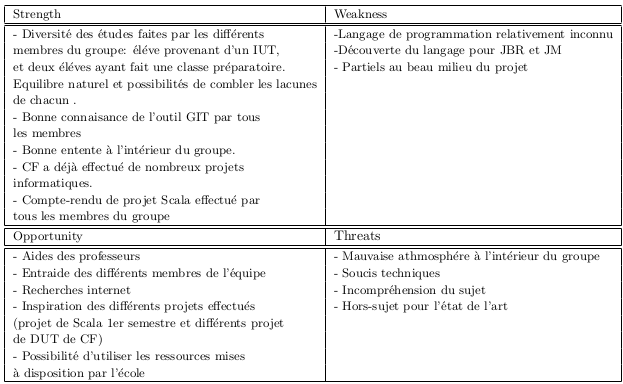
\includegraphics[scale=1]{SWOT.png}
    \caption{Matrice SWOT}
\end{figure}
    
\newpage
\subsection{Diagramme de Gantt}
Pour pouvoir nous organiser, répartir les tâches et imposer des dates limites, l'ensemble du groupe s'orienta naturellement vers un GANTT. 
Le diagramme ne contient que les premières semaines du projet, car, d'un commun accord, nous avons décidé de laisser les quelques semaines avant rendu sans date limite ou travail imposé par personne, car cela nous permettrait d'être beaucoup plus réactif. Pour pallier au manque d'organisation qu'implique le délaissement du Gantt, de nombreux "stand-up meeting" ont été organisés pour pouvoir se tenir au courant de l'avancement du projet.\\
Pour la version papier où la visibilité du Gantt ne sera pas optimale, voici le descriptif de ce dernier:

\begin{itemize}
        \item Création du parseur de document : 19/03/18 au 06/04/18
        \item Création de la structure de données film : 02/04/18 au 06/04/18
        \item Recherche de document pour l'état de l'art : 19/03/18 au 30/03/18
        \item État de l'art: 02/04 au 10/05/18
        \item Création de l'interface graphique du 23/04/18 au 10/05/18
        \item Création de TableFilm : 23/04/18 au 10/05/18
\end{itemize}

\newpage
\begin{figure}[!h]
    \centering
    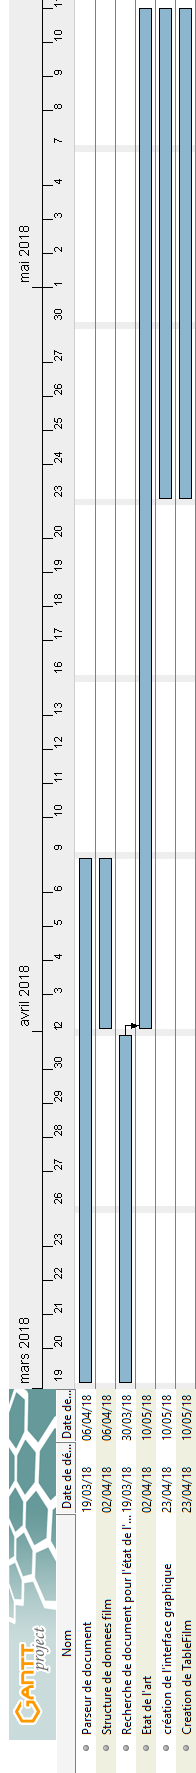
\includegraphics[scale=0.25]{Projet_c_rotateLeft.png}
    \caption{Diagramme de Gantt}
\end{figure}
\newpage
\subsection{Trello}
L'outil en ligne Trello nous a permis de nous organiser au cours du projet, de suivre l'avancement des étapes de chacun et de visualiser le travail à faire, en train d'être fait et fait.
\begin{figure}[!h]
    \centering
    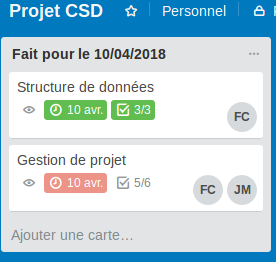
\includegraphics[scale=1]{CaptureTrello.png}
    \caption{Diagramme de Gantt}
\end{figure}
\newpage

\subsection{Comptes-rendus de réunion}
\subsubsection*{Réunion du 06/03/2018 à 16h00}
\paragraph*{Ordre du Jour}
\begin{enumerate}
\item Élection du chef de projet
\item Répartition des outils de Gestion de Projet à réaliser
\item Avancement du projet
\end{enumerate}

\paragraph*{Élection du chef de projet}\mbox{}

Colin FLORY est élu à l'unanimité chef de projet
\paragraph*{Répartition des outils de Gestion de Projet}\mbox{}

Colin FLORY devrait faire pour la réunion du 13/03 la matrice SWOT du projet, Jean-Baptiste RENAULT le GANTT à condition d'avoir le sujet. Juliette MAUSSION devra rédiger le compte-rendu de cette réunion.
\paragraph*{Avancement du projet}\mbox{}

Pour la prochaine réunion, le sujet venant d'être donné, chacun des membres devra faire des recherches autour des systèmes de recommandation.

\subsubsection*{Réunion du 27/03/2018 à 16h}
\paragraph*{Ordre du Jour}
\begin{enumerate}
\item Mise au point de l'état de l'art
\item Répartition des tâches
\end{enumerate}
\paragraph*{Mise au point de l'état de l'art}\mbox{}
Colin Flory a trouvé deux liens exploitables pour l’état de l’art, un en anglais, "A Collaborative Filtering Recommendation Algorithm Based on User Clustering and Item Clustering ", orienté un peu plus mathématiques qui permettra d’avancer dans les algorithmes plus facilement, et un en français, une thèse de l’Université de Lorraine, qui permet de poser les bases et de comprendre le décor des systèmes de
recommandation.
\paragraph*{Répartition des tâches}\mbox{}
Les deux documents trouvés seront à lire par tous les membres, en particulier la thèse de l’UL.
J-B. Renault et J. Maussion devront établir l’état de l’art à partir des deux documents et d’autres qu’ils trouveront pour pouvoir commencer à coder rapidement la suite du projet.
C.Flory rédigera un script permettant de récupérer les données disponibles pour le projet sur les films à recommander.

\subsubsection*{Réunion du 10/04/2018 à 16h}
\paragraph*{Ordre du Jour}
\begin{enumerate}
\item Mise au point de l'état de l'art
\item Structures de données
\end{enumerate}
\paragraph*{Mise au point de l'état de l'art}\mbox{}
L'état de l'art a avancé, mais est très imprécis, il manque des formules et des outils concrets qui nous permettraient de commencer réellement à coder en sachant où l'on va. Les bases des systèmes de recommandations et des différentes approches sont là, mais survolées pour le moment.
\paragraph*{Structures de données}\mbox{}
Colin FLORY continue de travailler sur la hashmap. 

\subsubsection*{Réunion du 11/05/2018 à 13h}
\paragraph*{Ordre du Jour}
\begin{enumerate}
\item Mise au point de l'état de l'art
\item Structures de données
\item Interface graphique
\end{enumerate}
\paragraph*{Mise au point de l'état de l'art}\mbox{}
Juliette MAUSSION a à nouveau avancé l'état de l'art, qui est maintenant bien plus complet, le cheminement est bien plus clair et mis à part la partie sur l'évaluation des systèmes de recommandations cela devrait suffire pour faire l'intégralité du projet sans rechercher davantage. 
\paragraph*{Structures de données}\mbox{}
Les structures de données sont bien avancées, et Colin FLORY a commencé le système de recommandation. 
\paragraph*{Interface graphique}\mbox{}
Jean-Baptiste RENAULT a avancé dans l'interface graphique en s'appropriant l'utilisation des Widgets et de GTK. En continuant, on va pouvoir se rapprocher d'une interface adaptée à notre projet.
\newpage

\section{Participation aux tâches au sein du groupe}
    \par Une case vide signifie que la personne n'a pas travaillé sur ce point.\\
    \begin{tabular}{|c|c|c|c|}
        \hline
        Tâches & FLORY Colin & Juliette MAUSSION & Jean-Baptiste RENAULT \\
        \hline
        \hline
        Gestion de projet & 6 heures  &  & \\
        \hline
        Parseur & 20 heures & & \\
        \hline
        Structures de données & 17 heures & & \\
        \hline
        Afichage graphique & & & 39 heures\\
        \hline
        Affichage en ligne de commande & 4 heures & & \\
        \hline
        Algorithme de recommandation & 8 heures & & \\
        \hline
        Option -json& & 22 heures & \\
        \hline
        Rédaction du rapport & 15 heures & 5 heures & 9 heures \\
        \hline
        Rédaction des comptes-rendus & \multirow{2}{*}{}&\multirow{2}{*}{} &\multirow{2}{*}{} \\ 
        de réunions & & 3 heures & \\
        \hline
        Travail sur l'état de l'art & & 20 heures & 3 heures\\
        \hline
        Total & 72 heures & 50 heures & 51 heures\\
        \hline
    \end{tabular}
\newpage
\bibliographystyle{plain}
\bibliography{biblio.bib}


\end{document}